\documentclass{article}
\usepackage{graphicx}
\usepackage{float}
\usepackage{fullpage}
\usepackage{array}
\usepackage{pdflscape}
\usepackage{multirow}
\usepackage{bibentry}
%\nobibliography*
\usepackage[T1]{fontenc}
%\usepackage{lscape}
%\usepackage[parfill]{parskip}
\usepackage{listings}
\setlength{\extrarowheight}{4pt}

\graphicspath{{./images/}}

\floatstyle{boxed}
\restylefloat{figure}

\begin{document}

\lstset{language=sh,
        frame=single,
        breaklines=true,
        basicstyle=\small\ttfamily,
        columns=fullflexible}


\begin{titlepage}
\begin{center}
\vfill
\hfill
\\[2cm]
\textsc{\LARGE University Of Waterloo}
\\[1cm]
\textsc{\LARGE ECE 355}
\\[2cm]

\hrule
\hfill
\\[0.5cm]
\textsc{\huge Software Requirements Specification}
\\[0.5cm]
\textsc{\huge GARTH}
\\[0.5cm]
\textsc{\huge Green, Aware, and Responsive Total Home}
\\[0.5cm]
\hrule
\hfill
\\[1cm]
\textsc{\LARGE Group 16} \\[0.4cm]

\begin{minipage}{0.4\textwidth}
\begin{flushleft} \large
Ben Ridder \\
Casey Banner \\
Zack MacLennan
\end{flushleft}
\end{minipage}
\begin{minipage}{0.4\textwidth}
\begin{flushright} \large
brridder \\
20299452 \\
20305946 
\end{flushright}
\end{minipage}


\vfill

{\large \today}
\end{center}
\end{titlepage}

\tableofcontents
\listoffigures
\lstlistoflistings
%\listoftables

\section{Purpose and Scope of Implementation} % Zach
% 10%
% State the purpose of the document and its intended audience. Refer to the
% requirements and design documents.

% Summarize what portion of the design was actually implemented in the
% prototype. Describe the main use cases supported by the implementation. List
% any significant requirements not implemented due to time constraints.

The purpose of this document is to discuss the software implementation that was
created and presented to the evaluators. This software was based on the structure
and guidelines as stated by the software requirements specification document and
software design document that had previously been drafted. This document is
intended to be able to bridge these previous documents with the piece of software
that had been implemented. It will give insight into many of the various design
decisions as well as any changes that were made to the software in which the
implementation had varied from the design as stated in the SDD. It will discuss
testing strategies and results, error handling and what errors were accounted
for, how to install a run the software, as well as the extensibility of the design.

The intended audience of this document are the evaluators of the software project.
They need to be able to make connections with the two previous software documents,
and this document will strive to meet that criteria by discussing the topics mentioned
above. Through reading this implementation report they should be able to see
what subset of the overall design was implemented, what changes were made to
the portions that were indeed implemented, and how to install and run the software
should they feel the need to evaluate it from a closer perspective.

The portion of the design that was implemented was a somewhat small but very
significant portion of the overall proposed design. The implemented design
included a server mock-up with transient storage meant to emulate the server
design. The system controller as presented in the software design document was
realized in the implementation, and communicated with the server and the mobile
applications through the communication stack via sockets. There were two mobile
applications implemented, one of which ran on the Android platform and the other
ran on iOS in order to emulate the cases where a user had either an iPhone or an
Android smartphone. Finally a basic GUI was designed to emulate the triggering
of sensors positioned around the home. These sensors were designed to be able
to replicate the use cases that were implemented. The use cases that were
accounted for originated from the software requirements specification and include:

\begin{itemize}
\item Arming and disarming the system through use of a keypad
\item Door sensor events to detect intruders if system is armed
\item Window intrusion detection if system is armed while a window is opened
\item Irregular thermostat behaviour and over-temperature conditions
\item Flood detection if basement water levels reach an unsuitable level
\item Motion sensors to detect movement in the home while the system is armed
\end{itemize}

These use cases were made as consistent as possible with the software requirements
specification with the exception of added robustness for error cases and extra
functionality.

\section{Changes to the Design} % Casey or Ben???
% 10%
% Summarize any changes that were required to the design specified in the
% Design Document, and jusity the design deviations.

% left out hardware interface: sockets instead
% Moved subscribeToEvent to eventManager3
% Simple logging functionality
% Sending startup and shutdown events

There were not many major changes required in the implementation of the system.
The major one was the change from using radios to using sockets to communicate
between the controllers and the simulated hardware. This was out of necessity
as there was no plans to implement hardware sensors in the initial release. A
more minor change was moving the function
\texttt{subscribeToEvent(event:Event)} from the controllers described in
Figures~5.2, 5.3, and 5.4 in the design document to the event manager found in
Figure~5.5. The design of controllers and event manager makes it so that it
does not make sense for the controller to subscribe to events on itself, but
rather call into the event manager to do so.

The next change was to add a simple logging functionality using text files and
JSON. This will allow for quick searching of triggered events which will assist
in debugging. It will also be simple to add the logged events to a database
once it is implemented via a script. Finally, the last change was the addition
of sending controller start up and shut down events to the server and log
files. This provides an easier means to see the status of the controllers and
the errors associated with them through the mobile applications.

\section{Transformation to Implementation} % Ben
% 10%
% Summarize how the design was mapped to the implementation. Consider the
% process model, process communication, storage schema, and other areas were
% implementation decisions were made.

The classes of the system were mapped from the class diagrams in the UML of the
design document in figures of Chapter~5. 

The controllers are run on separate threads so that they can all respond to
events in a timely manner. The event manager, which the controllers and devices
use to communicate through, is run on two separate threads, the main thread and
an additional one, in the same process as the controllers. This was to allow
for the event manager to be able to enqueue events from the controllers without
blocking sending of the events to the controllers.

Database storage was omitted from this release, but there is a simple log of
the events stored with the controllers in JSON format. This log can be easily
parsed into a database with a script once a database has been implemented into
the system.

The process model was kept simple. The controllers talked to the event manager.
The event manager and the devices talked to each other through sockets. A
sensor console user interface was created to assist in sending sensor events
through the sockets to the event manager and eventually the controllers. The
system controller handled what to do for each event type. If an alarm event
needed to be fired off, then the system controller instantiated it and sent it
to the event manager to be sent to the alarm devices and alarm controller.
Every event handled by the system controller was sent to a web server through
JSON-RPC. 

A web server maintained a list of events in memory. These events were fetched
by the two mobile applications for iOS and Android platforms. Events are
viewable on either application depending on what the user has. The iOS
application, due to the overhead required to properly store and display data,
was written in a similar manner to the system itself. Each event type is
represented as a class with proper usage of inheritance. The Android
application, with it's more flexible libraries, was able to use a list data
structure and display the data without first creating models. Both applications
can be easily extended as required by future needs.

\section{Testing Strategy} % Casey 
% 10%
% Identify the general approach taken to testing. For example, discuss the
% manner in which subsystems were tested individually through unit testing and
% in which the system was tested as a whole through integration testing.
% Identify the main subsystems and interfaces included in the test plan.
% Describe the test environment, including emulation of hardware devices.

Several testing strategies were employed during the development of
GARTH. Firstly, test-driven development was used during the initial
phases of development and any time new classes or functionality was
added. Secondly, larger tests were written that verified
interoperability of the various GARTH components. Finally, a sensor
test console program was created for integration testing purposes.

Test-driven development was used to ease development by reducing the
risk of introducing bugs when adding new code and changing existing
code. In this strategy, when a developer was about to add some new
functionality, a unit test for that functionality was added
first. This way, the developer can interpret the software spec once,
write the test, then concentrate on adding the functionality to pass
the test. This reduces the time that the developer spends context
switching between reading the software specification and the code
itself. Another added benefit of this testing strategy was that every
line of code in the project was executed at some point by the test
suite; this means that any refactor that was made could easily be
verified by simply re-running the test suite.

Larger automated tests were written that verified that the different
parts of GARTH communicated correctly. Any time that a communication
channel between two components was implemented by the developer, an
automated test for that communications channel was added. For example,
when socket connections were added to the communications stack,
automated tests were added that verified that the data sent via
sockets was correct. Having automated tests with a larger scope
allowed for large refactors to be made during development with minimal
risk.

Finally, in order to test the system's behaviour in response to the
various inputs it could receive, a test sensor console program was
created. This program consisted of a GUI with buttons to trigger each
type of Event in the system, as well as text fields to customize the
specific fields in each Event subclass. This sensor console was used
to verify that the logic in the various state machines was
correct. The console was also used during the project demo to
demonstrate the high level functionality of the system.

\section{Error Handling}
% 10%
% Describe potential and realistic faults that could occur in the
% implementation and how the system prevents, detects, mitigates, and/or
% recovers from failure. For instance, describe whether the implementation
% performs error checking on user input, recovers from interrupted
% commmunication, or handles component failure.

The GARTH implementation contains both error handling as well as
logging functionality. However, several potential faults
exist. Firstly, faults can occur within the communication stack if
there is a problem with any of the socket connections. Secondly, there
are potential faults if the remote server is inaccessible. However,
GARTH does include user input validation and prevents faults related
to erroneous input.

The communications stack contains exception handling logic to mitigate
the risk of failed or interrupted socket connections. If an error
occurs while establishing a client socket, an exception is thrown by
the underlying Python socket library this exception is handled by
GARTH by printing an error message. This behaviour is the same if an
existing socket connection encounters some other error; an exception
is raised by the sockets library and handled by GARTH.

If a connection cannot be opened to the external webserver, GARTH will
log an error message, but it will not attempt to reconnect to the
server.

The test sensor console used in GARTH testing contains several fields
where the user can enter arbitrary input. This input determines what
appears in the various fields of the Event objects that are created
and sent by the sensor console. However, the fields of the Event
objects have specific types. To avoid potential faults, the sensor
console attempts to convert the user input to the required type, and
if that conversion fails, will not send the particular Event. For
example, if the field is required to be an integer, but the user
enters a string, the type conversion will fail and the particular
Event that field corresponds to will not be sent.

The software requirements specification and software design document specified
specific error-cases and how the system would handle such failures.
Unfortunately some of these error cases weren't handled in the implementation
of the software that was demonstrated, simply because many of the systems
were emulated in ideal circumstances. For example, since the sensors were
represented by simple buttons on the demo GUI, there wasn't any option for
forcing the sensors to fail to see how they would behave in an error condition
such as communication failure or low-battery. However, if these systems were to
have been implemented, the user would have been notified of these fault 
conditions via a minor alarm alert on the mobile application. The user would
see this alert and investigate it by checking the sensor themselves or
contacting a GARTH representative. Adding this error case would have been trivial,
albeit it was not implemented.

\section{Test Results}
% 20%
% Summarize what testing techniques were performed on the implementation.
% Consider tests that pertain to functionality, interfaces, boundary
% conditions, resource handling, performance, load handling, and system
% integration. Do not include full test case descriptions, but rather, describe
% the tests that were executed in general terms.

Unit testing was extensively used while GARTH was being
implemented. Every method in every class within the GARTH
implementation has a test case. This test case will provide inputs and
ensure that the function produces the correct outputs or changes in
state. 

A main goal during the testing of GARTH was to achieve 100\% test
coverage. This means that every line of code in the GARTH
implemenation is executed at some point during the run of the test
suite. This statistic is particulary important for an interpreted
language like Python because some code is not parsed until it is run,
therefore some errors may not appear until runtime. If every line of
code is run during the test suite, the developer can be assured that
none of these errors exist in the codebase. The test coverage report
for the GARTH implementation can be found in Figure~\ref{fig:test_coverage}.

\floatstyle{plain}
\restylefloat{figure}
\begin{figure}[hp]
    \centering
        \caption{Test Coverage Results}
        \scriptsize
        \setlength{\unitlength}{2.0em}
        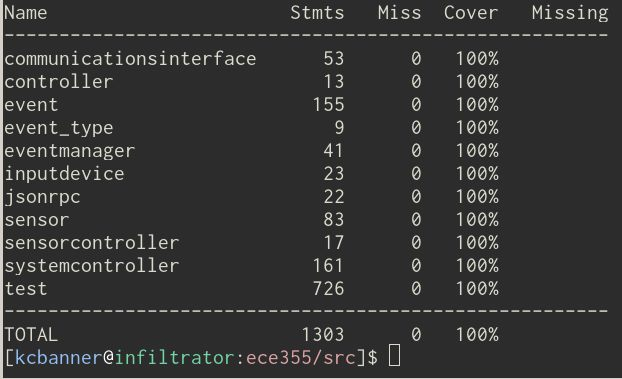
\includegraphics[scale=0.5]{test_coverage.png}
        \normalsize
    \label{fig:test_coverage}
\end{figure}
\floatstyle{boxed}
\restylefloat{figure}


\section{Outstanding Issues} % Zach
% 10%
% List any outstanding faults, deficiences, or missing features, and make
% recommendations on how they should be addressed in the final version.

The implemented design was light on error-handling, as much of the
main focus was in regards to getting robust functionality in place. As
a result, the intended error cases for sensor communication failure
and sensor low-battery were not in place when the subset of the design
was implemented. Although there was no way to emulate sensor failure
in the demo, this error case is trivial to put in place and will be
ready for the final version.

Another missing feature for the implemented software was distinct user
authentication. Although the access array and access control matrix was fully
explained in the software design document, user ID and password authentication
was not put in place for the implementation of the subset. However, for the
purposes of the software demo unique user experiences were emulated with the
fact that mutliple mobile applications were able to run simultaneously. This
showed how the software would behave given that more than one user was
manipulating the system at once. Creating a scheme for logging into these 
applications will be implemented for the final version of the design by 
creating a log-in screen for the mobile app that queries the access array
and control matrix for ID and password verification as well as setting permission
levels to each user.

Finally, the implemented software that was presented did not have persistant
storage for the server. Instead, the logs were cleared every time the server
was reset. This was not an issue for the case of the demo as the server remained
active the entire time, however it did not adequately show how the final version
would have behaved in the case of an unexpected server reboot. In order to fix
this, a simple XML file could be created that would be able to provide us with a
more permanent storage solution in the form of a database.

\section{Build and Installation Instructions}
% 10%
% Provide a brief outline of the steps required for compiling, installing, and
% running the implementation given a copy of the submitted source code. List
% any development tools and libraries that are required.

No compilation is required for the controller, console, and web server.
Installation is as simple as running the correct programs with several
parameters such as listening ports, peers, and remote URLs. The following
development tools and libraries are required for running the
system:
\begin{itemize}
\item Python 2.7 
\item Mox -- for running the test suite
\item wxPython -- for the sensor controller
\item node.js ($\ge$ v0.4) -- for running the web server
\end{itemize}

Listing~\ref{install-instructions} details the instructions for running the
various components of the system. It is assumed that all of the components are
running on the same computer using port \texttt{8000} to communicate through
sockets between peers. The server is located at \texttt{127.0.0.1} on port
\texttt{3000}.

\lstset{caption={Running instructions},
        label=install-instructions}
\begin{lstlisting}
$ ./run_controllers -r http://127.0.0.1:3000 -l 8000 & 
$ ./sensor_console.py -p localhost:8000 &
$ cd server
$ node app.js
\end{lstlisting}

The mobile applications do need to be compiled and downloaded to device. For
the iOS application, a device needs to have a valid provisioning profile and
development account in order to download the beta application to it. The
Android version works without any special permissions.

\section{Extensibility} %Zack
% 10%
% Recommend any functional and non-functional improvments to make in the final.
% version of the implementation to be released or a subsequent version. These
% may address use cases that have already been described, or have been
% considered following completion of the Design Document. For instance,
% consider whether the system may be made more reliable, perform better, scale
% to more users, function with new types of components, or be more accessible.
% Give specific examples consistant with the present implementation.

Since the implementation was a subset of the design as presented in the design
document, there is much left to be implemented that would add significant scale
to the system. For example, the mobile apps could be extended to add more
robust functionality as well as provide the user with more control over the
GARTH home system and its configuration. In its current iteration, the mobile app
is very light on settings and functionality. By adding proper user authentication
using the access control matrix, users with adequate permissions could easibly
configure the system through the mobile app which would communicate with the
server.

As mentioned above, having more error handling could improve the reliability
of the system. If a system were implemented for detecting sensor failure,
low-battery, or a communication problem then the system would be less likely
to fail in an ungraceful manner. The user would be notified that a failure has
occurred and would be able to get the sensor fixed or replaced in a timely manner.
This would ensure a much better user experience overall.

Another way to demonstrate the extensibility of the GARTH design would be to
examine the simplicity at which a new sensor or component could be added to the
system. The way the different sensor classes inherit from the sensor class and
the fact that they include a sensor ID field allows for a new sensor of an 
existing type to be added easily. For example, if the front door is fitted with
a door sensor and another one were to be added to the back door, this would
be pretty much a plug and play procedure due to the nature of the class structure
as implemented with the sensor ID system.

\end{document}
